\documentclass[10pt]{beamer}

\usepackage[utf8]{inputenc}

\usetheme{Madrid}
% \usecolortheme{beaver}
\usepackage{xcolor}
\usepackage{listings}
\graphicspath{ {figures/} }

\lstset{
    basicstyle=\fontsize{6}{7}\selectfont\ttfamily\color{black},
    commentstyle=\color{gray},
    frame=single,
    numbers=left,
    numbersep=5pt,
    numberstyle=\tiny\color{gray},
    keywordstyle=\color{blue},
    showspaces=false,
    showstringspaces=false,
    stringstyle=\color{green},
    tabsize=2
}

\title{Android Testing}
\author{William Royall Drumheller, Eric Tanner Reed}
\date{16APR2019}

\begin{document}

\begin{frame}
\titlepage
\begin{center}
Proudly created using \LaTeX
\end{center}
\end{frame}

\begin{frame}
\frametitle{Testing Structure}
\begin{itemize}
    \item Small Tests
        \begin{itemize}
            \item small scale Unit tests
            \item e.g. testing that a counter increments correctly
            \item run locally on a development machine, without an emulator
        \end{itemize}
    \item Medium Tests
        \begin{itemize}
            \item test the integration between multiple components or classes
            \item e.g. testing classes that access a file system or network
            \item typically need Android environment resources
            \item need to run on an emulator or physical device
        \end{itemize}
    \item Large Tests
        \begin{itemize}
            \item deal with system level and end user components
            \item e.g. testing the UI functionality, including the \textit{MainActivity}
            \item typically need Android environment resources
            \item need to run on an emulator or physical device
        \end{itemize}
\end{itemize}
\end{frame}

\begin{frame}
    \frametitle{Testing Structure}
    \center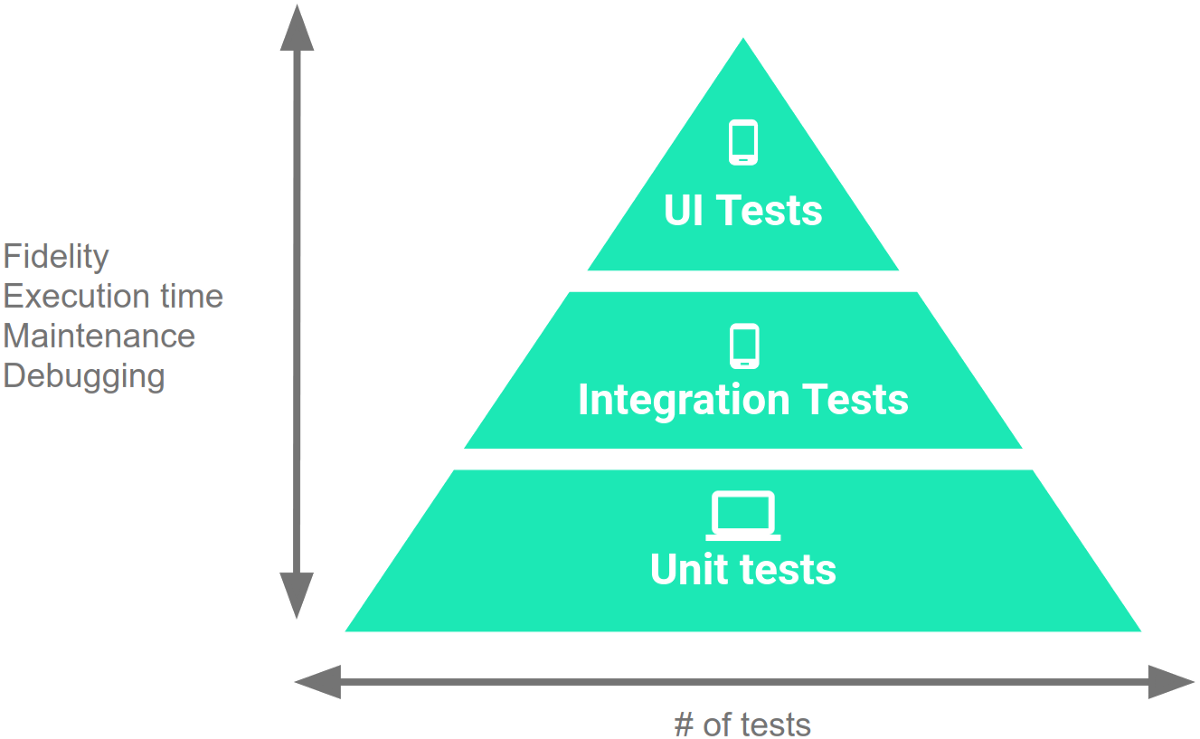
\includegraphics[scale=0.25]{3rd_party/pyramid_2x}
    \tiny\emph{https://developer.android.com/training/testing/fundamentals}
\end{frame}

\begin{frame}
    \frametitle{Development and Testing Workflow}
    \center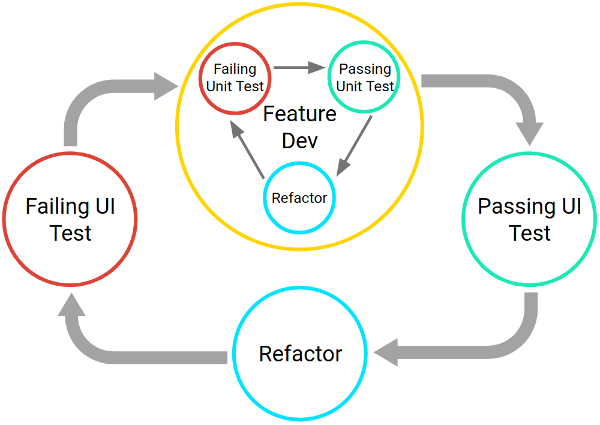
\includegraphics[scale=0.5]{3rd_party/testing-workflow}
    \tiny\emph{https://developer.android.com/training/testing/fundamentals}
\end{frame}

\begin{frame}
\frametitle{Why Do I Care?}
\begin{itemize}
    \item Test Driven Development (TDD)
    \begin{itemize}
        \item Start with a failing test, implement the bare minimum to make it pass, repeat
        \item Reduce code bloat and feel confident that when all tests pass, the job is done
        \item Legacy code is not sustainable, so writing well-tested code is key
    \end{itemize}
    \item Problem!
     Testing can be very, very slow!!!
     \begin{itemize}
        \item We need to optimize our workflow by running tests as quickly as possible
        \item Seconds of delay or interruption can hinder productivity
        \item Small (unit) tests should be run frequently
        \item Large (UI) tests should be run sparingly, since they require an emulator
     \end{itemize}
\end{itemize}
\end{frame}

\begin{frame}
    \frametitle{So... What Do We Feel Like Building?}
    \center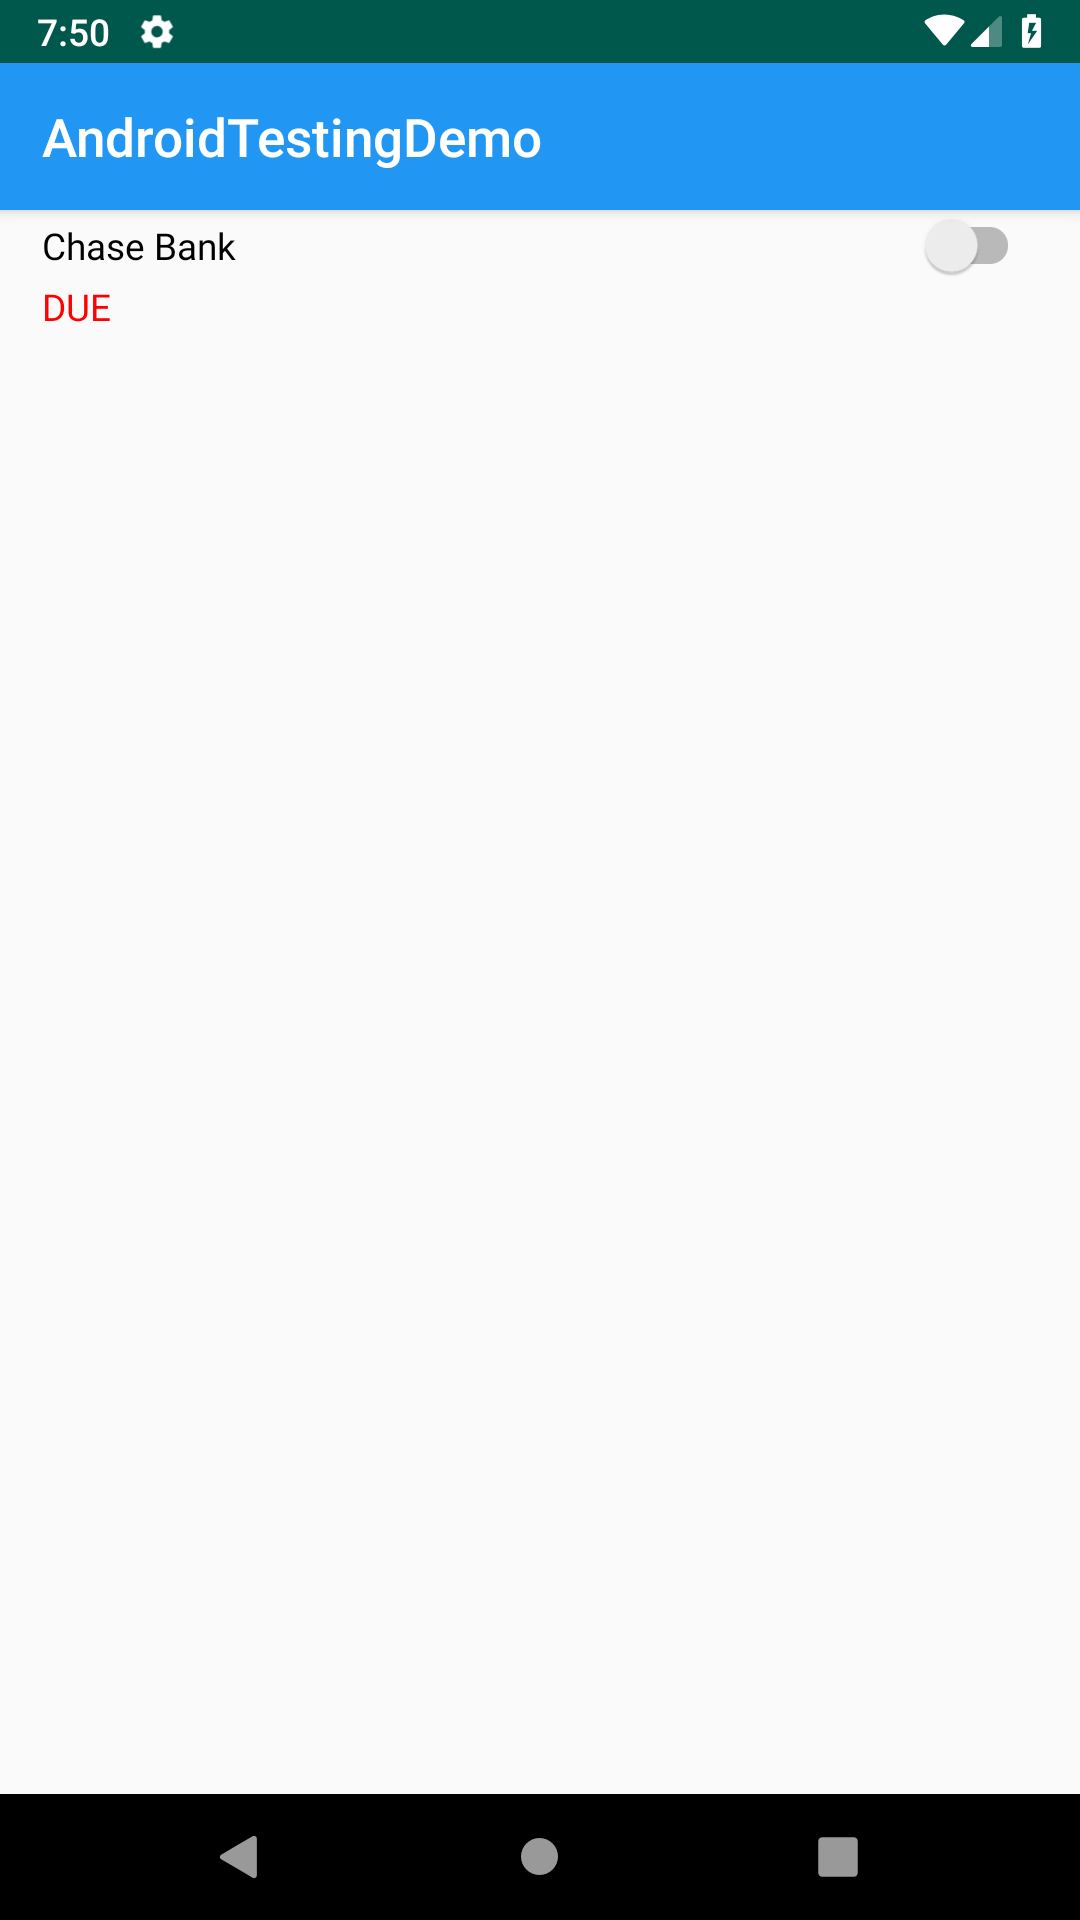
\includegraphics[scale=0.11]{ui_initial_state}
\end{frame}

\begin{frame}
    \frametitle{What Do We Feel Like Building?}
    \center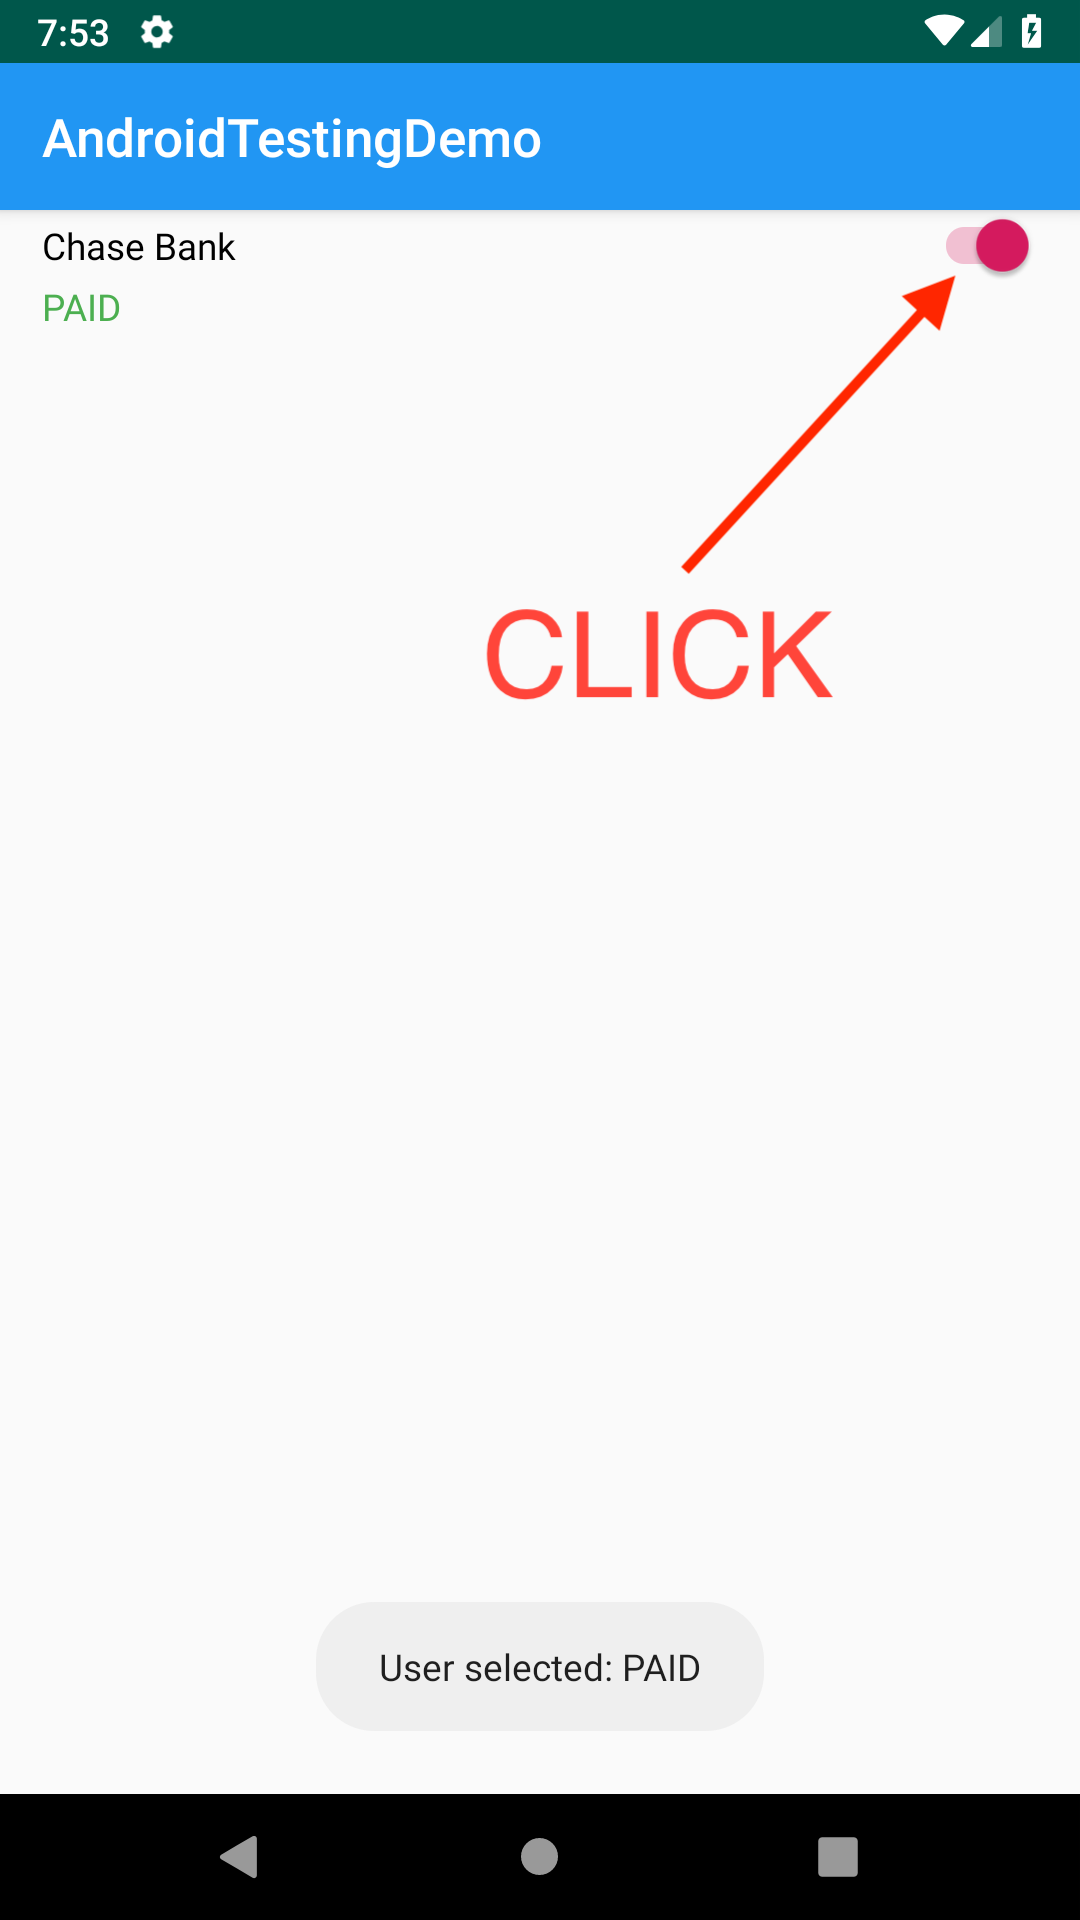
\includegraphics[scale=0.11]{ui_after_click}
\end{frame}

\begin{frame}
    \frametitle{What Do We Feel Like Building?}
    \begin{itemize}
        \item Demo of Application
        \item Feel free to clone and follow along!
        \item https://github.com/RoyallDesigns/AndroidTestingDemo
    \end{itemize}
\end{frame}

\begin{frame}
\frametitle{Tools of the Trade}
We are going to explore the following Testing Tools needed in our project:
\begin{itemize}
    \item \textit{AndroidX} and \textit{Espresso}
    \item \textit{mockito}
    \item \textit{Robolectric}
\end{itemize}
\end{frame}

\begin{frame}
    \frametitle{AndroidX and Espresso}
    \center
\includegraphics[scale=0.15]{3rd_party/espresso}
    \begin{itemize}
        \item \textit{AndroidX} provides testing libraries that can be used with \textit{JUnit}
        \item \textit{AndroidX} also provides \textit{Espresso}
        \item \textit{Espresso} provides a library for automated UI testing
        \item Automated tests of the UI are much more scalable than manual testing
    \end{itemize}
    \tiny\emph{https://developer.android.com/training/testing/espresso}
\end{frame}

\begin{frame}
    \frametitle{AndroidX Migration}
    \center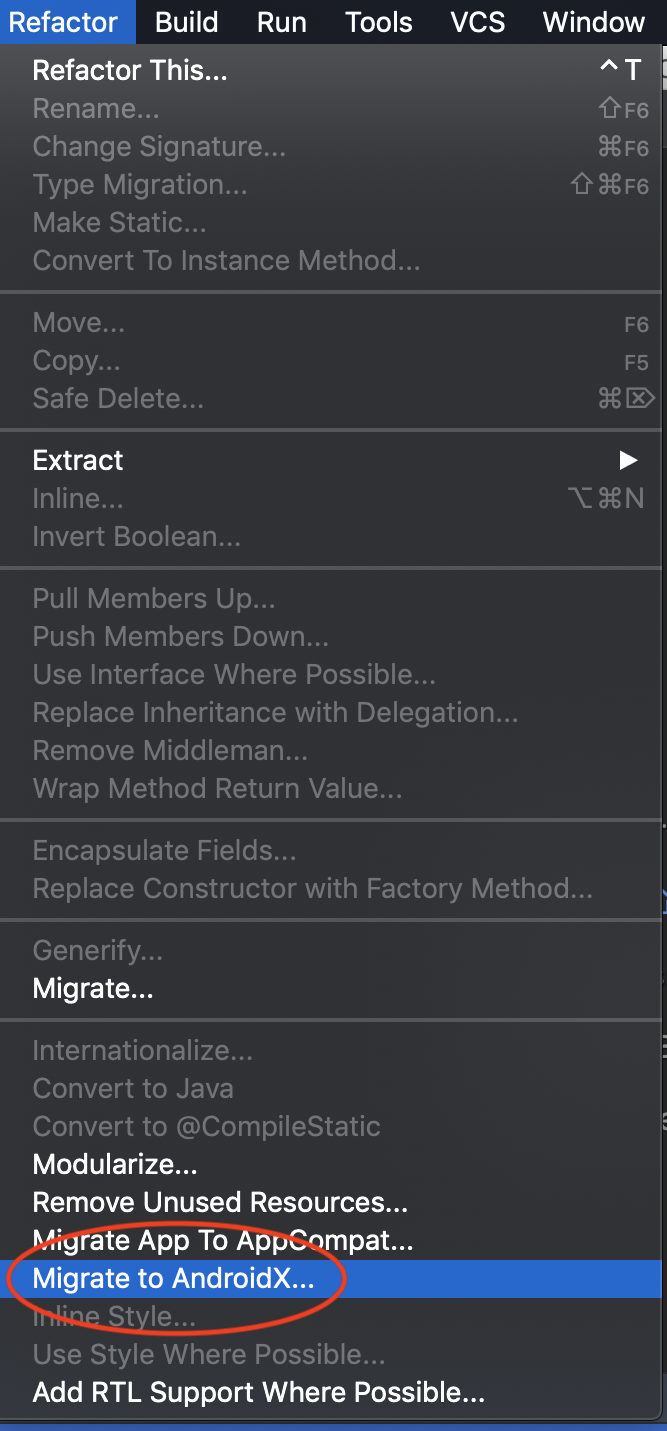
\includegraphics[scale=0.32]{androidx_step1}
\end{frame}

\begin{frame}
    \frametitle{AndroidX Migration}
    \center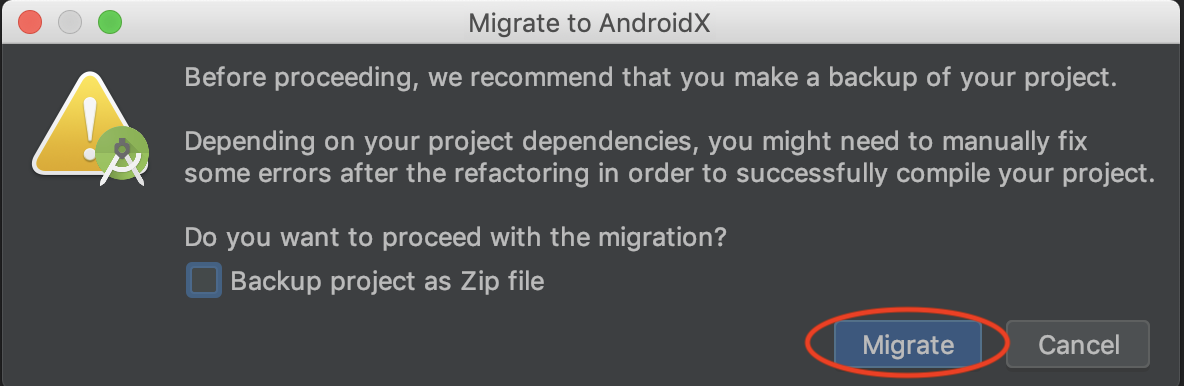
\includegraphics[scale=0.5]{androidx_step2}
\end{frame}

\begin{frame}[fragile]
\frametitle{Adding JUnit, AndroidX, and Espresso}
\begin{lstlisting}[caption={build.gradle}]
    dependencies {
        implementation fileTree(include: ['*.jar'], dir: 'libs')
        .
        .
        .
        testImplementation 'junit:junit:4.12'
        testImplementation 'androidx.test:runner:1.1.0-alpha4'
        androidTestImplementation 'androidx.test:runner:1.1.0-alpha4'
        androidTestImplementation 'androidx.test:rules:1.1.0-alpha4'
        androidTestImplementation 'androidx.test.espresso:espresso-core:3.1.0-alpha4'
    }
\end{lstlisting}
\end{frame}

\begin{frame}[fragile]
    \frametitle{Using JUnit, AndroidX, and Espresso}
    \begin{lstlisting}[language=java, caption={ToggleStateBehaviorTest.java}]
        @RunWith(AndroidJUnit4.class)
        @LargeTest
        public class ToggleStateBehaviorTest {

            @Rule
            public ActivityTestRule<MainActivity> activityRule =
                new ActivityTestRule<>(MainActivity.class);

            @Test
            public void defaultSwitchStateIsOff() {
                onView(withId(R.id.chase_switch)).check(matches(isNotChecked()));
            }

            @Test
            public void defaultTextViewIsDue() {
                ViewInteraction interaction = onView(withId(R.id.chase_text_view));
                interaction.check(matches(hasTextColor(R.color.due)));
                interaction.check(matches(withText("DUE")));
            }
    \end{lstlisting}
    Live Demo Time!
\end{frame}

\begin{frame}
    \frametitle{Mockito}
    \center
\includegraphics[scale=0.15]{3rd_party/mockito_2x}
    \begin{itemize}
        \item \textit{Mockito} provides the framework to implement mocks
        \item Mocks are useful for "black-box testing", since they stub out functionality based on
        the interface
        \item The tester wants to provide a specific value that a method should return
        \item The tester defines basic, expected behavior without using a full blown object
        \item Mocks essentially prevent more overhead and more potential for failure
        \item Failures could stem from dependencies on implicit interfaces/behavior
    \end{itemize}
    \tiny\emph{https://site.mockito.org/}
\end{frame}

\begin{frame}[fragile]
    \frametitle{Adding Mockito}
    \begin{lstlisting}[caption={build.gradle}]
        dependencies {
            implementation fileTree(include: ['*.jar'], dir: 'libs')
            .
            .
            .
            testImplementation 'junit:junit:4.12'
            testImplementation 'org.mockito:mockito-core:2.26.0'
            androidTestImplementation 'org.mockito:mockito-android:2.26.0'
            .
            .
            .
        }
    \end{lstlisting}
\end{frame}


\begin{frame}[fragile]
    \frametitle{Using Mockito}
    \begin{lstlisting}[language=java, caption={StatePersistenceTest.java}]
        @RunWith(MockitoJUnitRunner.class)
        @MediumTest
        public class StatePersistenceTest {

            @Rule
            public TemporaryFolder temporaryLocation = new TemporaryFolder();
            @Mock
            private Switch mockSwitch;
            @Mock
            private Context context;

            @Test
            public void savesTrueSwitchStateToFileSystem() throws IOException {
                initMocks(this);
                when(mockSwitch.isChecked()).thenReturn(true);
                when(context.getFilesDir()).thenReturn(temporaryLocation.newFolder());

                SwitchStatePersistence persistence = new SwitchStatePersistence(context,
                    "state.save");
                String savedPath = persistence.saveState(mockSwitch);

                String result = new String(Files.readAllBytes(Paths.get(savedPath)));

                assertTrue(result.equals("true"));
            }
    \end{lstlisting}
    Live Demo Time!
\end{frame}

\begin{frame}
    \frametitle{Robolectric}
    \center
\includegraphics[scale=0.25]{3rd_party/robolectric}
    \begin{itemize}
        \item \textit{Robolectric} provides the framework test Android code without using an
        emulator
        \item \textit{Robolectric} also allows the user to forgo using mocks or spending overhead
        attempting to instantiate concrete Android objects
        \item Instead, the user may use "Shadow" objects, which can be used similarly to mocks
        \item Allows the user to run tests on the development machine using real Android framework code, as opposed
        to slowing down tests using an emulator
    \end{itemize}
    \tiny\emph{http://robolectric.org/}
\end{frame}

\begin{frame}[fragile]
    \frametitle{Adding Robolectric}
    \begin{lstlisting}[caption={build.gradle}]
        android {
            .
            .
            .
            testOptions {
                unitTests {
                    includeAndroidResources = true
                }
            }
        }
    \end{lstlisting}
\end{frame}

\begin{frame}[fragile]
    \frametitle{Adding Robolectric}
    \begin{lstlisting}[caption={build.gradle}]
        dependencies {
            implementation fileTree(include: ['*.jar'], dir: 'libs')
            .
            .
            .
            testImplementation 'junit:junit:4.12'
            testImplementation 'org.robolectric:robolectric:4.2.1'
            .
            .
            .
        }
    \end{lstlisting}
\end{frame}

\begin{frame}[fragile]
    \frametitle{Using Robolectric}
    \begin{lstlisting}[language=java, caption={ToggleStateBehaviorTestRobolectric.java}]
        @RunWith(RobolectricTestRunner.class)
        public class ToggleStateBehaviorTestRobolectric {

            @Test
            public void defaultSwitchStateIsOff() {
                ActivityController<MainActivity> activity =
                    Robolectric.buildActivity(MainActivity.class).setup();

                Switch chaseSwitch = activity.get().findViewById(R.id.chase_switch);

                assertFalse(chaseSwitch.isChecked());
            }
    \end{lstlisting}
    Live Demo Time!
\end{frame}

\begin{frame}
    \frametitle{What is Linting?}
    \begin{itemize}
        \item Now that we are done testing our app,
        how do we vest confidence in how well we wrote it?
        \item Well, the IDE tends to lint or check for possible suggestions to our code,
        as we write it
        \item Checks include syntax errors, spell checking, API issues, versioning issues, etc.
        \item Style recommendations are also provided
        \item Can force the IDE to lint our code on demand
    \end{itemize}
\end{frame}

\begin{frame}
    \frametitle{Linting}
    \center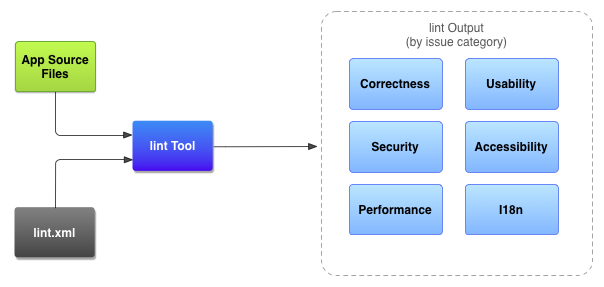
\includegraphics[scale=0.5]{3rd_party/lint}
    \tiny\emph{https://developer.android.com/studio/write/lint}
\end{frame}

\begin{frame}
    \frametitle{Your IDE... can Lint!}
    \center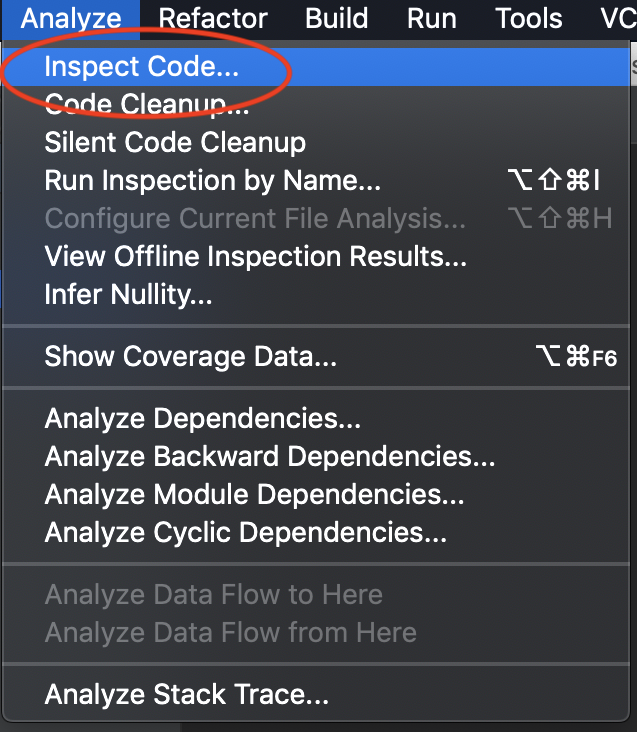
\includegraphics[scale=0.5]{lint_step1}
\end{frame}

\begin{frame}
    \frametitle{Your IDE... can Lint! (Live DEMO Time!)}
    \center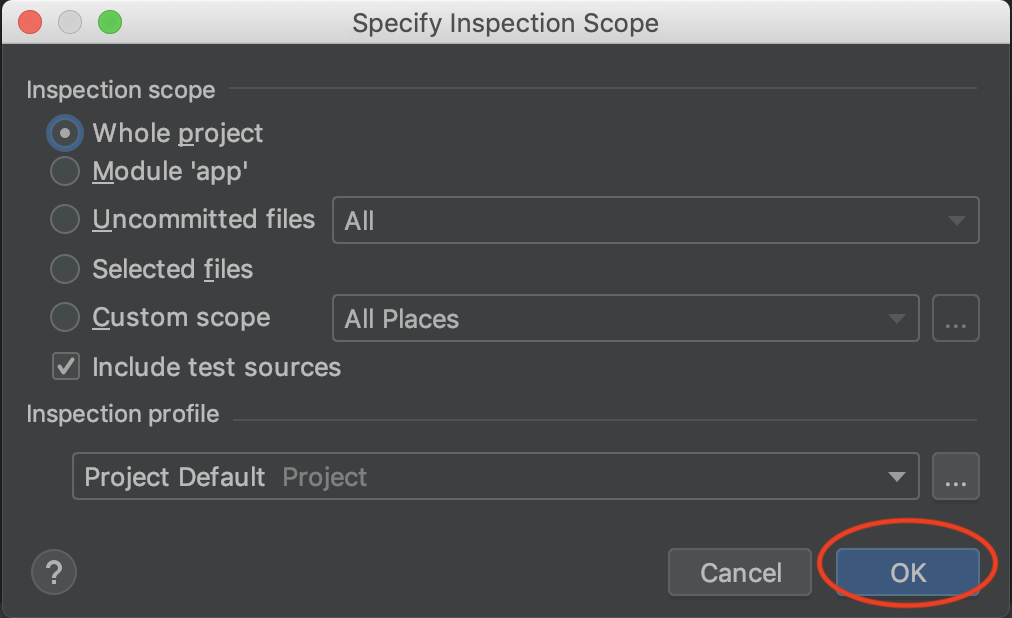
\includegraphics[scale=0.5]{lint_step2}
\end{frame}

\begin{frame}
    \frametitle{Questions, Concerns, Comments?}
    \begin{itemize}
        \small
        \item Anything to ask?
        \item Anything to be concerned with?
        \item Thoughts?
    \end{itemize}
\end{frame}

\begin{frame}
    \frametitle{References}
    \begin{itemize}
        \small
        \item https://developer.android.com/training/testing/fundamentals
        \item https://www.youtube.com/watch?v=pK7W5npkhho
        \item https://developer.android.com/training/testing/ui-testing/espresso-testing\#java
        \item http://robolectric.org/
        \item http://robolectric.org/writing-a-test/
        \item https://developer.android.com/studio/write/lint
    \end{itemize}
\end{frame}

\end{document}
